\chapter{Implementation}
This chapter presents the implementation of the design of the proposed summarisation system. The implementation presented in this chapter was used to assess the design’s limitations and efficacy for performing domain specific personalisation without the use of domain models. The methods used in the system design were implemented from their respective papers. Due to the availability of libraries available for text processing and topic modeling, this system was implemented using python 3.7.4 \citep{van2009python}. The existing methods selected to perform tasks of the system were implemented within python classes. Each python class encapsulates a number of methods from the identified design. The class structure for which the methods were implemented is unimportant to the system’s functionality, so this chapter will focus on the operations performed, using these classes. The functionality of the implemented system is presented in Figure \ref{designI}. The system uses three main processes to create extractive personalised summaries. Each process contains a set of relevant child processes. First, the Model and Corpus Generation process creates an annotated corpus and a topic model from a set of raw Wikipedia articles. Then the Query-based Document Retrieval process uses a query to retrieve relevant documents using the annotated corpus and topic model. Last, the Summary Generation process creates a summary from the sentences contained within the query relevant documents. Each of these processes implementations is presented in detail in sections of this chapter. 

\begin{figure}[h]
    \centering
         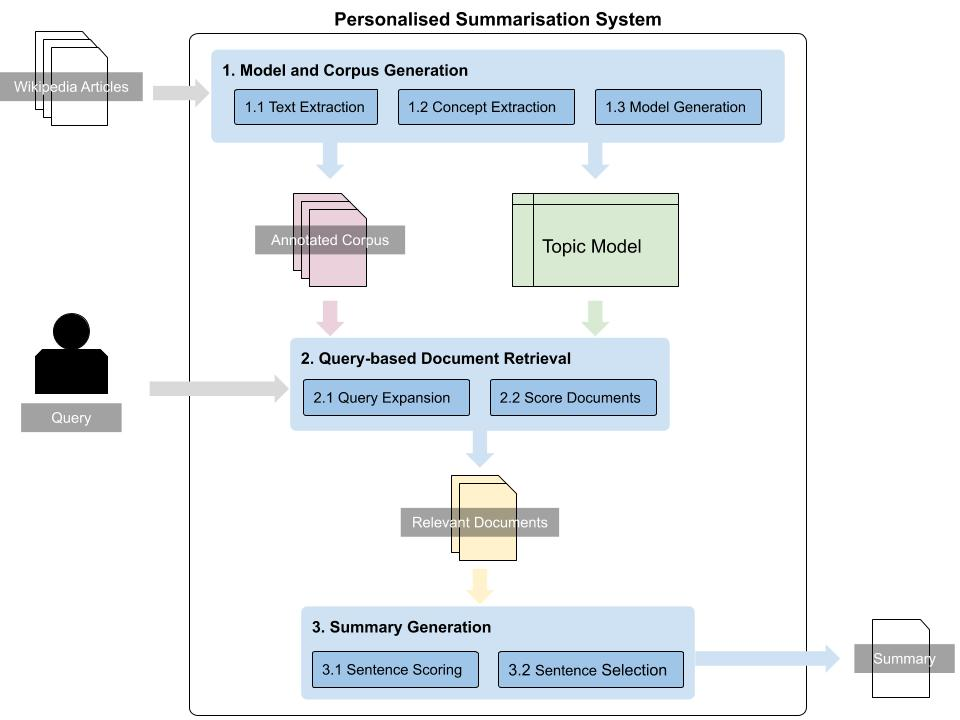
\includegraphics[width=0.70\textwidth]{Figures/System_Design_Overview.jpg}
          \caption{Design of system implemenation processes.}
           \label{designI}
\end{figure}

\section{Model and Corpus Generation}
The Model and Corpus Generation process of the system produces a meta-data annotated corpus and topic model. This process of the system is done via three child processes, text extraction from source material, concept extraction from text, and the creation of an annotated corpus used in the creation of a topic model. These processes are broken down in Figure \ref{modelDesign}.

\begin{figure}[h]
    \centering
         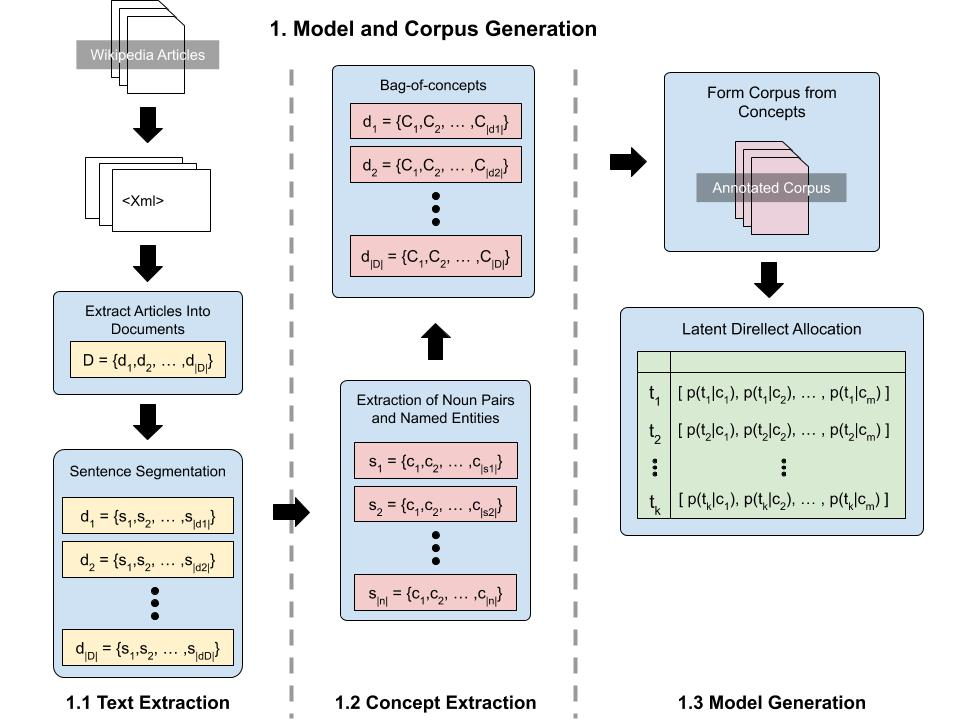
\includegraphics[width=0.70\textwidth]{Figures/System_Design_Model_Gen.jpg}
          \caption{Process of Model and Corpus Generation.}
           \label{modelDesign}
\end{figure}
Where $D$ is the document set extracted from articles, and $|D|$ is the number of documents extracted from source articles. $s_i$ is sentences in each document and $|d_i|$ is the number of sentences in each document. $c_i$ are the concepts extracted from $s_i$ and $|s_i|$ is the number of concepts in sentence $s_i$. $C_i$ is the set of concepts in sentence $s_i$. $t_i$ are the latent of topics determined by the model given $k$ is the number of topics. $m$ is the number of different concepts found in corpus $D$.

\subsection{Text Extraction}
This process takes a set of Wikipedia articles and extracts their textual content to be used in the creation of the corpus which is used in the formation of the topic model. Articles were downloaded using Wikipedia’s export system\footnote{\url{https://en.wikipedia.org/wiki/Special:Export}}. The export consists of a XML document that contains articles based on a given list of article titles. The list of articles were those that were in the category of “Watergate Scandal” on Wikipedia. The Wikipedia XML dump was processed using a python script called WikiExtractor\footnote{\url{https://github.com/attardi/wikiextractor}}. This script produces a simplified XML document from a Wikipedia dump that contains a <doc> element for each article. Each <doc> element contains just the text within the article, where every line in the doc tag is a paragraph in the article. Each <doc> element also contains a id, url, and title attribute unique to the article it contains. 

\begin{lstlisting}[language=XML]
<doc id="2102647" url="https://en.wikipedia.org/wiki?curid=2102647" 
title="Huston Plan">
    The Huston Plan
</doc>
\end{lstlisting}

\subsubsection{Producing Documents From Articles}
From the preprocessed Wikipedia xml, the text of each article contained in <doc> is extracted. As discussed in Section \ref{subsec:3.5.2}, to increase accuracy of the topic model and to respect the styling of Wikipedia articles, each paragraph (represented as a single line in the <doc> element) was treated as separate documents. The method to perform this was implemented in the Corpus class in Corpus.py. The Corpus class gets the preprocessed cml, from WikiExtractor.py. Using the python package BeautifulSoup \citep{richardson2007beautiful}, each <doc> in the simplified XML is iterated over. Each line (i.e. paragraph) of text, in a <doc> element, is used in the creation of a Document object, defined in Corpus.py. Each document object stores the title, url, id, as well as the paragraph number it corresponds to. The Document object that is created is then appended to a list of documents that are stored in the Corpus class. The list of all documents is annotated so sentences used in the summary can be referenced by the article they come from with a provided link to that article.

\begin{lstlisting}[language=Python]
def generate_docs(self, filename):
    with codecs.open(filename, encoding='utf-8') as f:
        data = f.read()
        soup = BeautifulSoup(data, features="html.parser")
        documents = soup.find_all('doc')
        size = len(documents)
        for doc in documents:
            title = doc.get('title')
            url = doc.get('url')
            uid = doc.get('id')
            text = doc.get_text()
            text = re.split(r'\n+', text)
            # text is now split by paragraph
            text = list(filter(None, text))
            for index, t in enumerate(text):
                d = Document(t, title=title, url=url, uid=uid, paragraph=index)
                self.sen2con.update(d.sen2con)
                self.docs.append(d)
                self.concepts.append(d.concepts)
\end{lstlisting}
Each Document contains three data structures: sen2con, con2sent, and concepts. Each of these data structures are added to the Corpus object’s corresponding sen2con, con2sent and concepts data structures. Thus when the processing of documents is complete the Corpus class has three data structures that are representative of all the content given into the input of the system. These structures are:
\begin{itemize}
    \item \emph{sen2con} a python dictionary with every sentence in from the source articles is a key and a list of concepts as its value.
    \item \emph{con2sen} a python dictionary with every concept extracted from the text as keys and a list of corresponding sentences that contain that concept as a value.
    \item \emph{concepts} a list that contains a list of concepts for each document that is created, i.e. a bag-of-concepts.
\end{itemize}
\subsubsection{Documents and Sentence Segmentation}
Paragraphs from each Wikipedia article are passed into the Document class, defined in Corpus.py. Each document stores its content in three structures:
\begin{itemize}
    \item \emph{sen2con} dictionary which uses sentences as keys and list of concepts as values.
    \item \emph{con2sen} dictionary which uses extracted concepts as keys with a list of sentences that contain that concept as values.
    \item \emph{concepts} list which contains a list of concepts for each sentence in the document.
\end{itemize}
Sentences are segmented using the punkt sentence tokenizer \citep{kiss2006unsupervised} supplied in the nltk python python package \citep{bird2009natural}. This is a critical part of the system as sentences must properly be segmented to be reproduced in the final summary. The punkt tokenizer is based on an unsupervised algorithm to build a model for abbreviation words, collocations, and words that start sentences. The nltk package contains a pretrained model, which was used for sentence segmentation for each document. 

The document class makes use of the Concepts class defined in ConceptExtract.py. Each document uses this class to extract the concepts for each sentence determined by the punkt tokenizer. Once concepts are extracted they are added to the Document objects' three structures. This process is done in the gen\_con2sen() method used in the init method of the Document class.

\begin{lstlisting}[language=Python]
def gen_con2sen(self):
    con2sent = {}
    sent2con = {}
    list_sent = tokenizer.tokenize(self.text)
    for sent in list_sent:
        con_list = Concepts(sent).get()
        if con_list is not []:
            sent2con[sent] = con_list
            for con in con_list:
                if con in con2sent:
                    if sent not in con2sent[con]:
                        con2sent[con].append(sent)
                else:
                    con2sent[con] = [sent]
    concepts = []
    for key in sent2con.keys():
        for con in sent2con[key]:
            concepts.append(con)
    return con2sent, sent2con, concepts
\end{lstlisting}

\subsection{Concept Extraction}
Concepts are extracted from the creation of a Concepts object which is in the Concepts class in ConceptExtract.py. Plain text is first preprocessed using the word\_tokenize() method defined in the nltk package. This method splits off punctuation other than periods in the raw text. Then the tokenized text is passed to the concept\_chunk() method. The concept\_chunk method performs phrase chunking on the inputted text. Phrase chunking segments a sentence based on its subconstituents, such as noun (NP), verb (VP), and prepositional phrases (PP).  To perform chunking, the nltk class RegexParser was used. This class takes in grammar to use for the chunking of text. The grammar that was defined is the following:

\begin{lstlisting}
    NP: {<PP\$>?<JJ>*<NN.*>+}	#Noun Phrase
    P: {<IN>}				# Preposition
    V: {<V.*>}				# Verb
    PP: {<P> <NP>}			# PP -> P NP
    VP: {<V> <NP|PP>*}		# VP -> V (NP|PP)*
\end{lstlisting}

The output from the chunking produces a tree which is then traversed to extract terms with noun pair labels. An example of this is seen in Figure \ref{tree} which is a visualisation produced from the draw() method on the returned tree object from the RegexParser from chunking of the following sentence: “Nixon’s White House address”.
\begin{figure}[h]
    \centering
         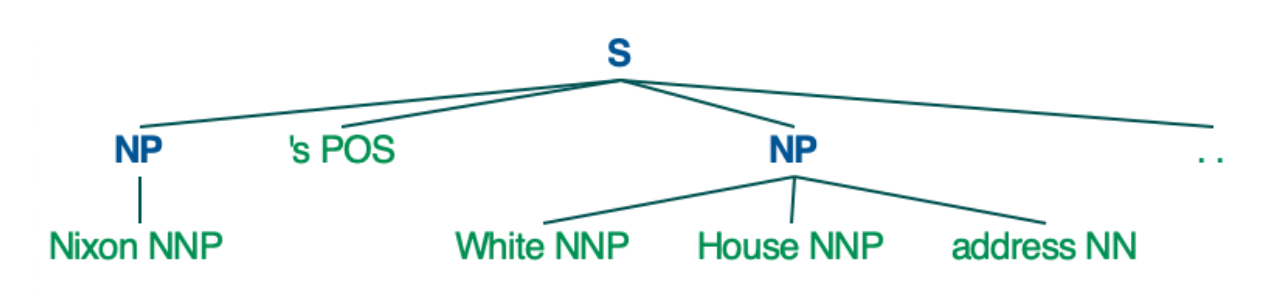
\includegraphics[width=0.70\textwidth]{Figures/tree.png}
          \caption{nltk tree formed from grammar by RegexParser.}
           \label{tree}
\end{figure}

The extracted nouns, represented by the “NP” label, in this example would be “Nixon” and “White House address”.

Named entities are also extracted from the text; this is done using the ne\_chunk() method in the nltk.chunk package. A named entity is considered to be names of people, locations, organizations, products, etc. Given the same input the ne\_chunk() method produces the following tree.
\begin{figure}[h]
    \centering
         
\includegraphics[width=0.70\textwidth]{Figures/treeNE.png}
          \caption{nltk tree formed from ne\_chunk().}
           \label{treeNE}
\end{figure}

Similarly named entities are those with a “NE” label, thus the named entities extracted are “Nixon” and “White House”. 

Both the named entities and the noun pairs are further processed to be all lowercase. The final set of concepts is the union between the list of found noun pairs and named entities. Concepts that are extracted from the example sentence are therefore [“nixon”, “white house address”, “white house”]. 

\subsection{Model Generation}
The Corpus.concepts object provides a bag-of-concepts representation. Corpus.concepts is a list that contains a list of concepts for each document. This representation and its benefits are discussed in Section \ref{subsec:3.5.1}. LDA uses this representation to construct a topic model from the corpus of documents. The construction of the corpus topic model is done by using the Model class in Model.py. The Model class uses the python package gensim \citep{rehurek2010software} to create a LDA model from the bag-of-concepts representation in Corpus.concepts. First a dictionary from the bag-of-concepts is created using the gensim.corpora Dictionary class. A dictionary is an object that maps each unique concept to a unique id. The Model class then uses this dictionary to produce a processed bag-of-concepts representation which contains a list that contains a list for each document. The list of a document contains tuples of concept id’s (from the dictionary) and their frequency in the document, see the following for a simple example.

\begin{itemize}
    \item \textbf{Bag-of-concepts}: [[“nixon”, “watergate”, “nixon”], [“impeachment”, “nixon”, “president ford”]]
    \item \textbf{Dictionary}: [(0,“nixon”),(1,”watergate”),(2,“impeachment”),(3,“president ford”)]
    \item \textbf{Processed bag-of-concepts}: [[(0,2), (1,1)], [(2,1), (0,1), (3,1)]]
\end{itemize}

Using the dictionary and the processed bag-of-concepts representation a model is formed using gensim.model.LdaModel(). The LdaModel uses a series of parameters to create a topic model, shown in Figure \ref{topicModel} provided from the python package pyLDAvis \citep{sievert2014ldavis}. The parameters used in the formation of the model are as follows:
\begin{itemize}
    \item \textbf{Corpus} – which is passed the processed bag-of-concepts object.
    \item \textbf{Id2word} – which is passed the dictionary object.
    \item \textbf{num\_topics} – passed the number of topics for model creation specified in the parameters of the Model class.
    \item \textbf{random\_state} – passed a static value of 100 which is used in the creation of the random priori using in model creation, this is static for model reproducibility.
    \item \textbf{update\_every} – passed a static value of 1. This specifies that parameters of the statistical model should be updated from every document passed into it.
    \item \textbf{passes} – passed a static value of 3, the number of passes over the corpus set of document
    \item \textbf{alpha} – set to auto, the alpha value is the priori belief for each topics’ probability, when set to auto the model learns an asymmetric prior from the corpus.
\end{itemize}

The crucial parameters for lda are the k number of topics latent topics and the hyper parameters such as alpha which describe the priori probability distribution between topics. There has been much work done to attempt to determine how to best select these parameters \citep{yau2014clustering,carter2016reading}, but there are no conclusive ways to determine the most optimal parameters when LDA is used in a wider system because certain model results from use of different parameters have different effects when LDA is used in larger system. Thus practical testing is the best way to determine these parameters \citep{suominen2016map}. The parameters here were assessed in an attempt to produce adequate models to be used in the summarisation system, but further evaluation could be performed to determine the optimal values for parameters with the effect of improving the personalised retrieval performance in the system.

\begin{figure}[h]
    \centering
         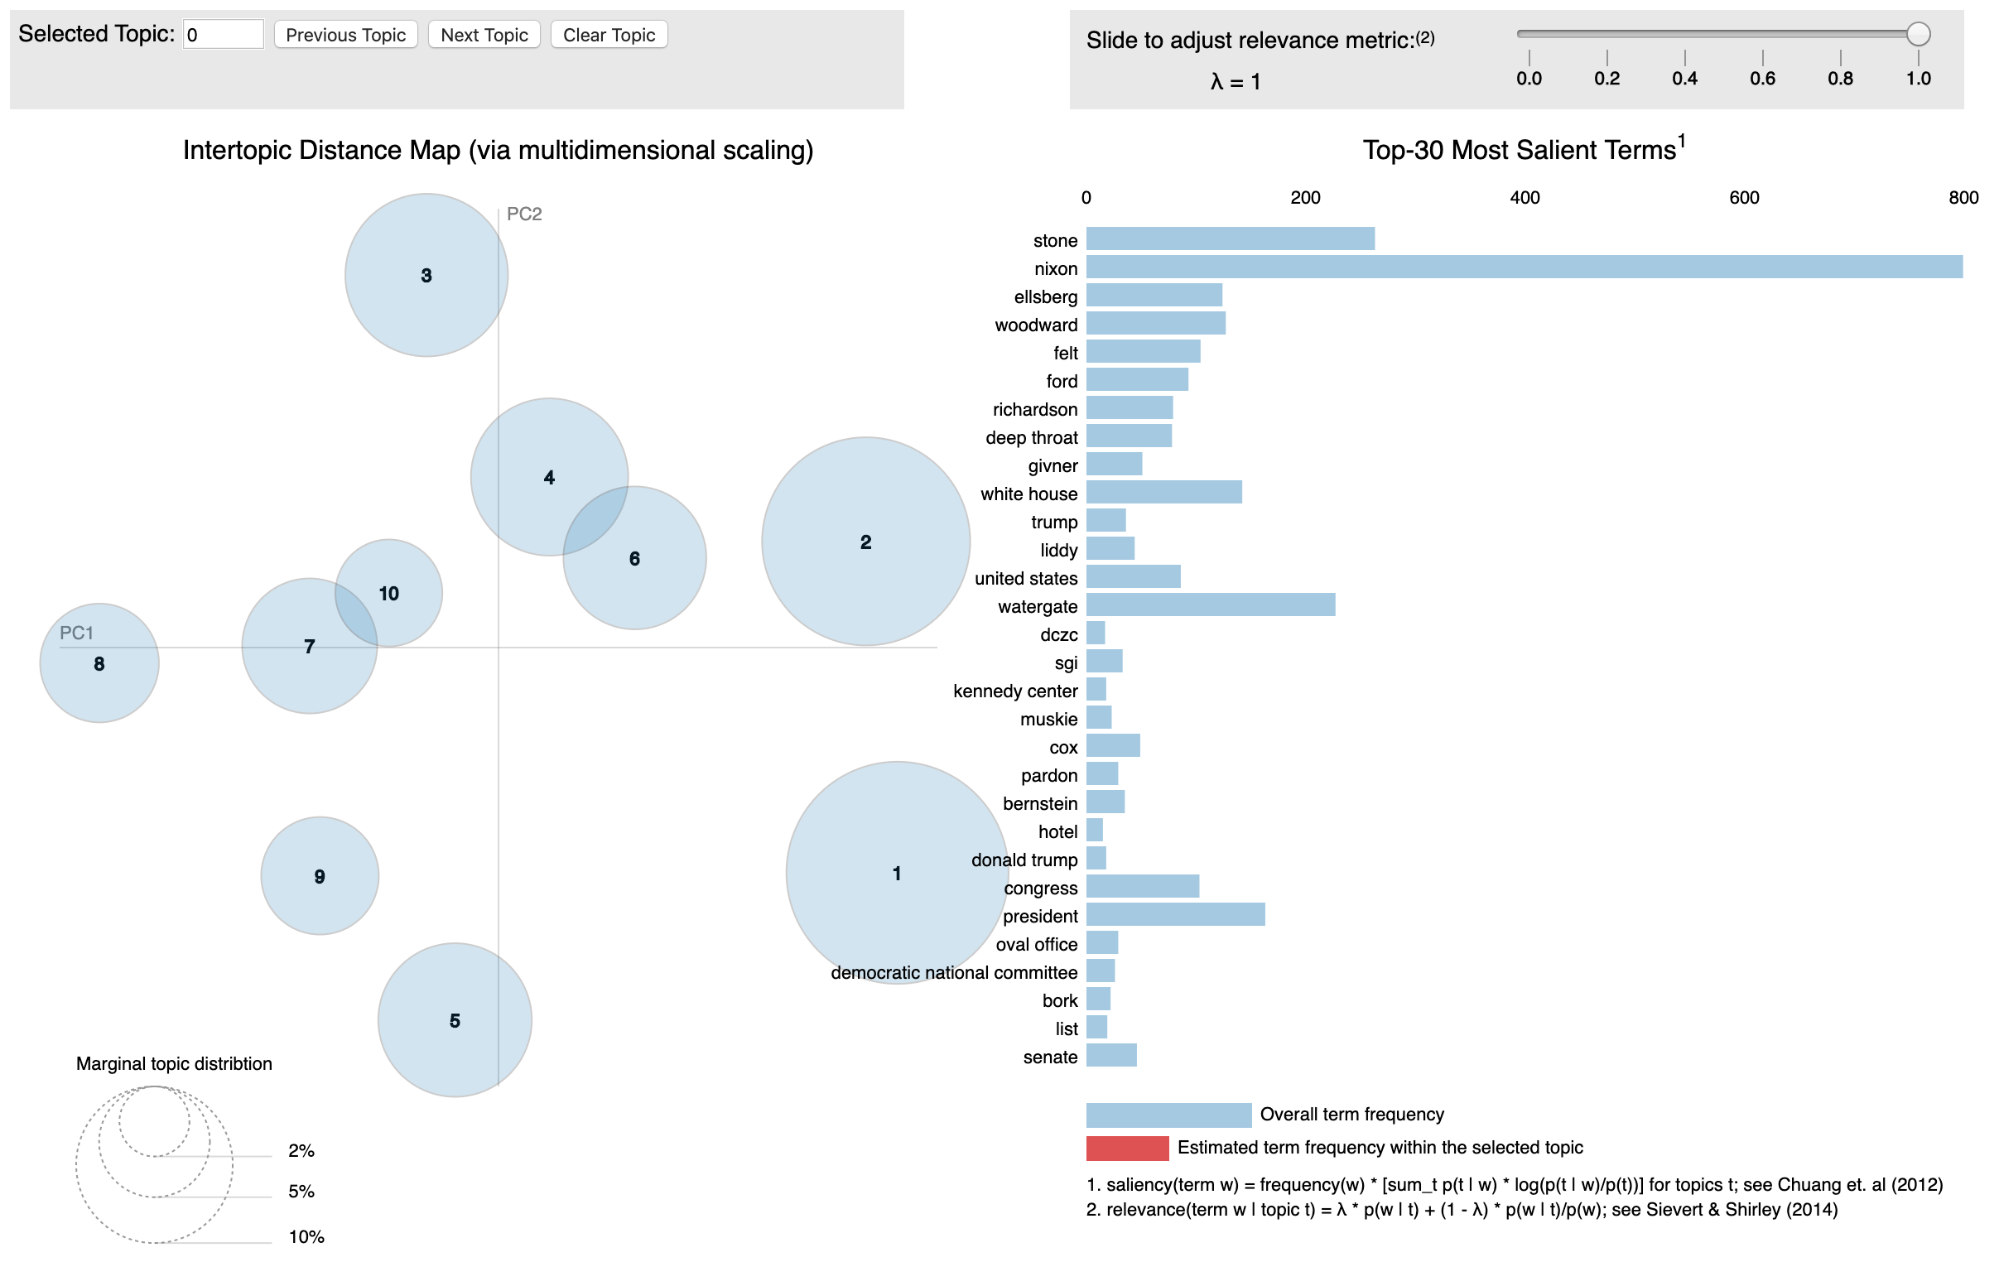
\includegraphics[width=1.0\textwidth]{Figures/ldamodel.png}
          \caption{pyLDAvis visualisation of topic model formed from Watergate Scandal Wikipedia articles.}
           \label{topicModel}
\end{figure}

\subsection{Summary of Model and Corpus Generation}
This series of processes work together to take the raw XML dumps of Wikipedia articles and create both Corpus object and Model object to be used in other parts of the summarisation system. The Corpus object parses articles into a series of Documents. Each Document object uses the Concepts class to create three structures: a dictionary modeling a mapping from sentences to concepts, a dictionary modeling a mapping from concepts to sentences, and a list of concepts found in the document. Each structure formed in a document gets added to the corresponding structures in the Corpus class, creating the same structures for all sentences and concepts in the input documents. The three data structures in the Corpus object will be used in all other aspects of the system to provide a variety of tasks for summarisation. The Model object creates and contains a LDA topic model, generated from the bag-of-concepts presentation in Corpus.concepts. This topic model will be used in retrieval of documents. The processes outlined in this section are the foundation for the rest of the processes performed in the summarisation system.

\section{Query-Based Document Retrieval}
The query-based document retrieval process of the system allows for the retrieval of a subset of the corpus set based on a specified query. A query relevant document set is passed into the summarisation process of the system, in order to provide a query based summarisation. This process of the system has two processes: query expansion and query document retrieval. The Query class, defined in Query.py, handles both the expansion of queries via cross concept chains as well as the retrieval of relevant documents in the corpus. Queries for this system are expressed using a sub set of concepts that are contained in the extracted set of document concepts. They are expanded from selecting all sentences containing the concepts given in the query to create a new document.  A specified number of additional relevant terms are selected based on the topic distribution of the new document. The expanded query is then used to determine a set of documents that are relevant based on the similarity of a query topic distribution and individual document’s topic distribution from the corpus. Documents with a similarity above a threshold are added to a list of documents to summarise in the summary generation process of the system.  These two processes and their implementation are discussed in this section.

\subsection{Query Expansion}
As discussed in Section \ref{subsec:3.5.3}, query expansion is a technique used to improve retrieval of documents. The output of expansion in this system are cross concepts chain queries done using the method presented by Li and Jin’s \citeyear{li2016cross} paper “Cross-document knowledge discovery using semantic concept topic model.” In \emph{2016 15th IEEE International Conference on Machine Learning and Applications (ICMLA)}. A query will contain a set of concepts that each relate to a various number of latent topics in the topic model. The aim is to add supplemental concepts to bolster the topic distribution in the original query, or to represent concepts from a hidden topic that connects topics discussed in the original query. This process uses a set of steps to produce a new expanded query topic distribution for query-based document retrieval. This implementation follows closely Li and Jin’s \citeyear{li2016cross} cross concept chain method.

\begin{figure}[h]
    \centering
         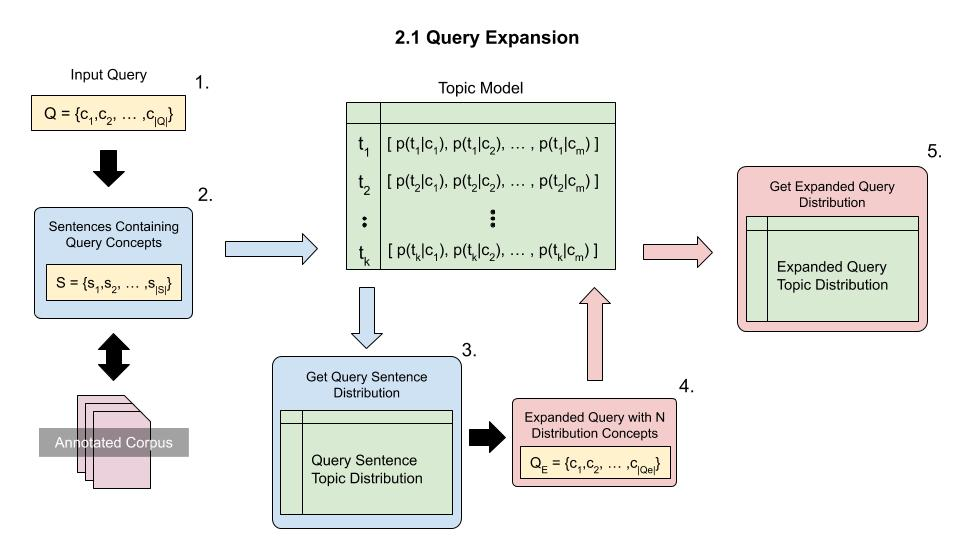
\includegraphics[width=1.0\textwidth]{Figures/System_Design_Query-Based_Retrieval.jpg}
          \caption{Process of expanding a query}
           \label{queryExp}
\end{figure}
Where $Q$ is the set of concepts that describe a query. $S$ is the set of sentences retrieved from the corpus that contains concepts given in $Q$. $Q_E$ is the union of the set of most relevant concepts extracted from the topic distribution of $S$ and the concepts from the original concept set $Q$.

Query expansion is done via the Query class defined in Query.py. A Query object is created by specifying a Corpus and Model object. These objects are created in the Corpus and Model generation process of the system. The expansion of an input query is done as the first step in the retrieve\_docs() method from a Query object. Expansion of queries is done via the get\_concept\_chain() method which uses the following parameters:

\begin{itemize}
    \item \textbf{concepts} – a query expressed as a list of concepts.
    \item \textbf{keywords} – a number specifying the final size of the expanded query.
\end{itemize}

This method follows the steps of the query expansion processes shown in Figure \ref{queryExp}. Step 2 in the processes uses the Corpus.con2sen object to find sentences that contain each of the concepts that are inputted in Step 1. The sentences are joined together to form a new document. This document is used in creating a new Model object in Step 3, producing a document specific lda model. Each topic found by this new lda model is iterated over in Step 4. For each of the topic\_ids in the new model are passed into the gensim.ldamodel method get\_topic\_terms(). This method takes topic\_id and number of terms and produces the top number of terms and their probabilities relating to a given topic\_id. The probability of the term relating to a query is given by  multiplying  the topic\_id probability and the probability of term relating to the topic\_id. Each of these top terms and their found probability are added into a list top\_n\_words. The top\_n\_words list is sorted and then iterated over. Words from the top\_n\_words lists are added to a list called cross\_chain\_query if they are not contained in the original query and the cross\_chain\_query length is less than the specified expanded length in the keywords parameter. The original query and  the new found words are combined to produce a cross concept chain expanded query. Step 5 uses this new query and passes it into the Model.lda\_model to get a topic distribution. This topic distribution is used in finding similar documents in the following query-based retrieval processes.

\subsection{Query-Based Document Retrieval}
This process takes an expanded query topic distribution and produces a subset of the corpus documents that are relevant to a query based examining the similarity of each document's topic distribution with the given query topic distribution. The topic distribution of any given document or query is a vector of latent topic\_ids and their corresponding probabilities of relating to the input. These vectors can be compared using a cosine similarity metric. The resulting documents can then be selected to be relevant based on a set threshold of similarity. This process is done in the Query class method retrieve\_docs():

\begin{lstlisting}[language=Python]
def retrieve_docs(self, concepts: [str], similarity = 0.80, query_len=10):
    # topic_dist = self.model.topic_dist(concepts)
    topic_dist = self.get_concept_chain(concepts, keywords=query_len)
    similar_docs = []
    count = 0
    for doc in self.corpus.docs:
        for sent in doc.sen2con.keys():
            sent_concepts = doc.sen2con[sent]
            doc_dist = self.model.topic_dist(sent_concepts)
            sim = cossim(doc_dist[0], topic_dist[0])
            if sim > similarity:
                count+=1
                similar_docs.append(sent)
    
    return similar_docs, topic_dist
\end{lstlisting}
retrieve\_docs() first expands a query using the method get\_concept\_chain(). The get\_concept\_chain() returns a topic distribution of an expanded query. For each Document in the Corpus object doc list, the concepts of the Document are passed into the Model objects topic\_dist method(). The similarity of the topic distribution of a Document and the expanded query is determined from using the gensim.matutils method cossim(). If the similarity is greater than the similarity threshold, the Document object text is added to a list that is returned at the end of execution. The returned list of document text is what is used in the summary generation process of the system discussed in the next section.

\section{Summary Generation}
The summary generation process of the system takes a set of relevant documents produced from the query-based document retrieval process and produces a summary. The summary process produces a summary via two processes: sentence scoring and summary generation. The implementations for both these processes are based on the method presented by Alguliev et al. \citeyear{alguliev2011mcmr} “MCMR: Maximum coverage and minimum redundant text summarization model” in \emph{Expert Systems with Applications}. Further discussion of this method is presented in Section \ref{subsec:3.5.4}. This method of summarisation treats summary formation as an optimisation problem, where the scores of combinations of sentences are combined in an attempt to maximise a summary score under the constraint of length. The matematical form of this problem is given in (\ref{mcmrFull}). Alguliev et al. approach is implemented within the Summary class in Summary.py. The Summary class takes in four parameters:

\begin{itemize}
    \item \textbf{doc} – a list of sentences that are considered for summarisation.
    \item \textbf{corpus} – a Corpus object created on all documents.
    \item \textbf{min\_len} – the minimum sentence length, in characters, to be considered for a summary.
    \item \textbf{num\_processes} – the number of python process used for sentence scoring.
\end{itemize}

\subsection{Sentence Scoring}
The Summary class calculates all considered combinations of sentences when initialised. This sentence scoring is done upon initialization to allow the scoring of combinations of sentences to be done concurrently. Before individual sentences are scored the list of sentences considered is pruned.

Sentences are removed from the list if they are: shorter than the length threshold specified in the min\_len parameter, redundant (the same sentence exists somewhere else in the list), or if the set of concepts extracted from the sentence is empty (accessed from Corpus.sen2con[sentence]). The pruned sentence list is then set to the Summary.sentences object (i.e self.sentences = pruned\_sentences). After the input sentences have been preprocessed the Summary class forms 3 data structures to be used in sentence scoring:

\begin{itemize}
    \item \textbf{self.sen\_con\_freq} – a python dictionary which uses each concept in the sentences list as key and a list of sentences that contain that concept as a value.
    \item \textbf{self.con\_freq} – a python dictionary which uses each concept in the sentences list as key a number occurrences of that concept in the set of sentences as a value.
    \item \textbf{term\_sent\_weights} – a dictionary of dictionaries where the parent dictionary uses each sentence as a key with a child dictionary as a value dictionary. The child dictionary uses concepts in a sentence as keys and the value is that terms tf-isf score calculated via (\ref{tfisf})
\end{itemize}

These structures are created in the method self.\_\_sent\_term\_weighting() in the Summary class. Once these structures are created a list of pairs of sentences is constructed and scored. This list of sentence pairs to be scored is created by the following for loop which is based on the double summation given from the mathematical formalisation:

\begin{lstlisting}[language=Python]
sentences_pairs = []
for i in range(0, len(sentences)-2):
    for j in range(i+1, len(sentences)-1):
        sentences_pairs.append((sentences[i], sentences[j]))
\end{lstlisting}

For each sentence pair the two scores for the respective pair are calculated using the generalised form of a similarity score, used in (\ref{mcmrGeneral}):
\begin{equation}
    score(s_i,s_j) = sim(D,s_i) + sim(D,s_j) - sim(s_i,s_j)
    \label{generalised}
\end{equation}

The similarity was calculated using two metrics: the cosine similarity and Normalised Google Distance (NGD). For each pair a score was calculated and stored in a dictionary.

The cosine similarity was calculated using the term\_sent\_weights object that was previously constructed. The three cosine similarity scores from (\ref{generalised}) were calculated using the cos\_sim function:

\begin{lstlisting}[language=Python]
def cos_sim(self, item1, term_sent_weights, con_freq, item2=None):
    item2_vec = []
    item1_vec = list((term_sent_weights[item1]).values())
    if item2 is None:
        item2_vec = list(con_freq.values())
    else:
        item2_vec = list((term_sent_weights[item2]).values())
    numerator = dot(item1_vec, item2_vec)
    denominator = (norm(item1_vec)*norm(item2_vec))
    similarity = numerator/denominator
    return similarity
\end{lstlisting}

Each sentence or document is first represented as a list by all the term weights for all the concepts that are contained within them. The cosine similarity is calculated from the dot product of the concept weights over the multiplication of the two vectors normalisation.

The normalised google distance for a sentence pair was calculated for three scores of the generalised similarity score formula (\ref{generalised}). The ngd score was calculated by ngd\_sim and ngd\_term method based on (\ref{ngdSent}) and (\ref{ngdTerm}) respectively:

\begin{lstlisting}[language=Python]
def ngd_sim(self, item1, n, sent_con_freq, con2sen, item2=None,):
    item2_con = []
    item1_con = con2sen[item1]
    if item2 is None:
       item2_con = list(sent_con_freq.keys())
    else:
       item2_con = con2sen[item2]
    ngd_sum = 0
    ngds_counted = 0
    for term1 in item1_con:
        for term2 in item2_con:
            ngds_counted += 1
            ngd = self.ngd_term(term1, term2, n, sent_con_freq)
            ngd_sim = math.exp(-ngd)
            ngd_sum += ngd_sim
   ngd = (ngd_sum/(len(item1_con) * len(item2_con)))
   return ngd

def ngd_term(self, t1, t2, n, sent_con_freq):
    t1_sen_count = len(sent_con_freq[t1])
    t2_sen_count = len(sent_con_freq[t2])
    t1_t2_sen_count = len([con for con in sent_con_freq[t1] if con in sent_con_freq[t2]])
    t1_log = math.log10(t1_sen_count)
    t2_log = math.log10(t2_sen_count)
    t1_t2_log = 0
    if(t1_t2_sen_count > 0):
        t1_t2_log = math.log10(t1_t2_sen_count)
    numerator = max(t1_log,t2_log) - t1_t2_log
    denominator = math.log10(n) - min(t1_log, t2_log)
    return (numerator/denominator)
\end{lstlisting}

From precalculating the scores of the sentence pairs in this implementation, the original maximization functions (\ref{mcmrFull}) is simplified to the following:

\begin{equation}
    Maximize \; f_{\alpha} = \sum_{i=1}^{n-1} \sum_{j=i+1}^n [\alpha(score_{cos}(s_i,s_j)) + (1-\alpha)(score_{ngd}(s_i,s_j))]x_{ij}
    \label{myMcmr}
\end{equation}

Inorder to reduce the time to generate a summary the scoring of sentence pairs is done concurrently. The list of sentence pairs is spit up evenly between a specified number of processes. These processes construct two dictionaries: one that contains the cosine similarity and one that contains the NGD scores of the senect pairs, where each sentence pair is a key to the respective score.

\subsection{Summary Formation}
The approach to the summary formation, the simplified maximisation function (15), given from precalculating the scores, must be formulated as an integer linear programming problem. The aim is to adjust the binary $x_{ij}$ variables to produce the highest scoring summary possible from the set of sentences. The resulting values of the $x_{ij}$ will identify the sentence pairs that should be contained in the final summary. The python package PuLP \citep{mitchell2011pulp} was used to implement (\ref{myMcmr}) as linear programming problem in the doc\_summary method:

\begin{lstlisting}[language=Python]
def doc_summary(self, sen_len=300, alpha=0.8):
    sentences = self.doc
    n_i = len(sentences) - 2
    n_j = len(sentences) - 1
    maxium_len = sen_len
    lp_problem = p.LpProblem('problem', p.LpMaximize)
    x_ij = p.LpVariable.dicts('xij', [(sentences[i],sentences[j]) for i in range(0, n_i) for j in range(i+1, n_j)], cat='Binary')
    constriant_len = p.LpConstraint(e=p.lpSum([(len(sentences[i]) + len(sentences[j]))*(x_ij[(sentences[i],sentences[j])]) for i in range(0, n_i) for j in range(i+1, n_j)]),sense=p.LpConstraintLE,rhs=300)

    objective = p.lpSum([ \
        (alpha * (self.find_cos_sim(i, j, sentences) * x_ij[(sentences[i],sentences[j])])) \
        + \
        ((1-alpha) * (self.find_ngd_sim(i, j, sentences) * x_ij[(sentences[i],sentences[j])]))
            for i in range(0, len(sentences)-2) for j in range(i+1, len(sentences)-1)])
    lp_problem += objective
    lp_problem += constriant_len

    maxium_summary_sent = []
    lp_problem.solve()

    summary_sent = {}
    variables_dict = {}
    variables_list = lp_problem.variables()
    for v in variables_list:
        variables_dict[v.name] = v.varValue
    variables_keys = list(variables_dict.keys())

    index = 0
    for i in range(0, len(sentences)-2):
        for j in range(i+1, len(sentences)-1):
            key = variables_keys[index]

            if variables_dict[key] > 0:
                summary_sent[sentences[i]] = ""
                summary_sent[sentences[j]] = ""
            index+=1

    return list(summary_sent.keys())
\end{lstlisting}

First a pulp LpProblem was initialised to maximise. Then a set of binary LpVariables was constructed representing pairs of sentences to be included in the summary. The length constraint was then added to the LpProblem specifying that the length of all sentence pairs to be included in the summary should be no longer than the specified sentence length. Then the objective was expressed in the same form as (\ref{myMcmr}) using the precalculated cosine and NGD similarity for sentence pair variables. Then the problem is solved by PuLP. The result is binary values of variables that represent sentence pairs to be included in the summary. These set of variables are iterated over to extract the set of sentences which should be included in the summary. The result is a list of sentences that the summary problem is maximised from.

\section{Summary}
The implementation of the processes of the system design have been described in this chapter. From the python classes the processes can be linked together to provide the functionality of the summarisation system. A simple example of how these classes are used is the following:

\begin{lstlisting}[language=Python]
corpus = Corpus([], filename='./WikiCorpus/WaterGateText/AA/wiki_00', regen=False)
concepts = corpus.get_concepts()
model = Model(concepts),topics=10)
query = Query(corpus, model)
Query_concepts = ["operation sandwedge", "political enemies", "caulfield"]
found_docs, query_topic_dist = query.retrieve_docs(query_concepts, similarity=0.80, query_len=20)
summary = Summary(found_docs, corpus)
summary_list = summary.doc_summary()
links = []
    for sent in summary_list:
        title, link = corpus.get_links(sent)
        if (title, link) not in links:
            links.append((title, link)) 
\end{lstlisting}

Implementing these methods into classes allows for a great deal of flexibility in constructing the methods to perform summarisation. From methods encapsulation they can individually be tested for correctness of implementation. The modularity of a class based implementation also allows for the parts of the system to be tested as single processes of the whole. The result is an implementation that produces the functionality outlined by the design that can be used to assess the system’s design extent of performing domain specific personalised summarisation without the use of formal ontologies.
